\documentclass[journal=jpccck,manuscript=article]{achemso}

\usepackage{hyperref}

\usepackage{siunitx}
\DeclareSIUnit\rydberg{Ry}
\usepackage{tikz}
\usepackage{paralist}
\usepackage[version=4]{mhchem}
\usepackage{booktabs}
\usepackage{rotating}
\usepackage{chngcntr}


\author{Pierre Beaujean}
\affiliation[Unamur]
{University of Namur, Theoretical Chemistry Lab, Unit of Theoretical and Structural Physical Chemistry, Namur Institute of Structured Matter, rue de Bruxelles, 61, B-5000 Namur (Belgium)}


\author{Benoît Champagne}
\affiliation[Unamur]
{University of Namur, Theoretical Chemistry Lab, Unit of Theoretical and Structural Physical Chemistry, Namur Institute of Structured Matter, rue de Bruxelles, 61, B-5000 Namur (Belgium)}
\email{benoit.champagne@unamur.be}

\title{Prediction of XPS binding energies for molecules grafted on calcium surfaces}

\def\dbe{\ensuremath{\Delta\text{BE}}}

\begin{document}
\maketitle

\section{Introduction}

Batteries represent a crucial technology for the transition to a climate-neutral society. Since their market introduction, lithium-ion batteries (LIBs) have evolved into a highly mature technology, currently utilized in a wide range of applications. Despite their established performance, LIBs face significant limitations that hinder their suitability for large-scale applications, primarily due to three fundamental issues:
\begin{inparaenum}[(i)] 
	\item limited availability of raw materials, 
	\item insufficient energy density, and 
	\item inadequate sustainability across an extended number of cycles. 
\end{inparaenum}

Addressing the second point can be achieved through the use of divalent cations, such as \ce{Ca^2+}. However, its elevated reactivity demands the design of specialized electrolytes to support a reversible mechanism. Additionally, detailed insight into the chemistry of the solid-electrolyte interphase (SEI) remains crucial.
In the literature, calcium-ion batteries (CIBs) utilize electrolytes such as dimethyl ether (DME), ethylene carbonate (EC), glyme, or tetrahydrofuran (THF), often in combination with weakly coordinating anions like \ce{BH4-} or \ce{BF4-} \cite{zhaoRevealingSolidElectrolyte2022,taghavi-kahaghPoweringFutureComprehensive2023}. Although both experimental \cite{melemedImpactDifferentialCa22023} and quantum chemistry \cite{hahnCriticalRoleConfigurational2020,liepinyaComputationalComparisonEther2021,pathreekerWhyTetrahydrofuranGood2021,yamijalaStabilityCalciumIon2021} studies on SEI formation exist, greater insight can be gained by combining experimental spectra with theoretical calculations.


X-ray photoelectron spectroscopy (XPS) is a surface-sensitive, quantitative spectroscopy that allows for the identification of elements within the material or at its surface. It belongs to the family of photoemission spectroscopies, where the energy of electrons emitted by the photoelectric effect is analyzed. Specifically, XPS uses a beam of soft X-rays ($\SI{100}{\electronvolt} < h\nu < \SI{10}{\kilo\electronvolt}$), enabling the probing of core electrons (low principal quantum number) \cite{stevieIntroductionXrayPhotoelectron2020}. The conservation of energy is described by the equation:
\begin{equation}
	h\nu = \text{BE} + E_{\text{kin}} + \phi, \label{eq:xps}
\end{equation}
where BE is the binding energy of the electron, $E_{\text{kin}}$ is the kinetic energy of the emitted electron (measured by the detector), and $\phi$ is the work function, which accounts for surface effects and detector contributions. Using a source of monochromatic X-rays (such as Al $K_\alpha$, $h\nu = \SI{1486.7}{\electronvolt}$), it is possible to determine BE from $E_{\text{kin}}$ \cite{vinesPredictionCoreLevel2018}. The binding energy depends on how tightly the electron is bound in its orbital, making it sensitive to the oxidation state and chemical environment of the originating atom. Generally, more electronegative surroundings result in higher BE, providing information on the atom's environment, much like chemical shifts in NMR. It is routinely used to gain understanding on the SEI composition, both experimentally \cite{melemedImpactDifferentialCa22023} and with calculations \cite{ebadiInsightsLiMetalOrganic2019}.  

This study investigates the XPS spectra associated with the degradation and polymerization of THF, using it as a model system. Various potential degradation products (Fig.~\ref{fig:THFdegradation}), as well as the polymerization into poly(tetramethylene ether) glycol (PTMEG), are examined on different calcium substrates, including calcium oxide and calcium hydride.


\begin{figure}
	\centering
	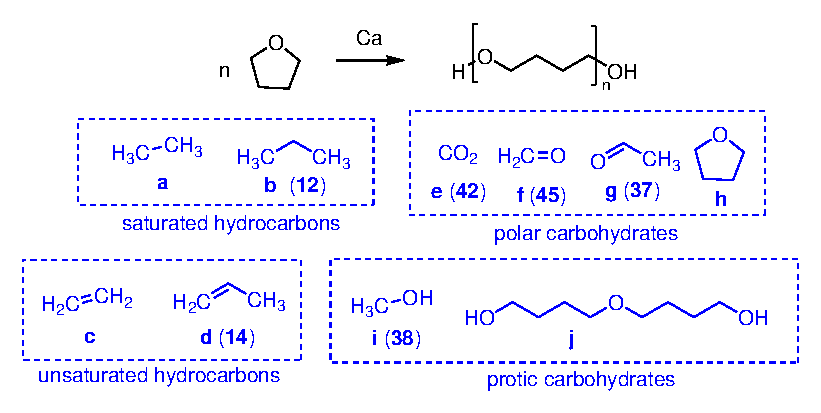
\includegraphics{Figure1}
	\caption{The main polymerization pathway of THF leads to PTMEG (black). \textbf{j} is used as a model for the PTMEG, while fragmentation can lead to (un)saturated hydrocarbons (\textbf{a}-\textbf{d}) or carbohydrates (\textbf{e}-\textbf{i}).}
	\label{fig:THFdegradation}
\end{figure}

\section{Theoretical methods}

From a quantum chemistry perspective, binding energy is akin to the ionization energy of core electrons:
\begin{equation}
	\text{BE}_i = E^{N-1}_i(\text{final}) - E^{N}(\text{initial}), \label{eq:dscf}
\end{equation}
where $E^{N}$ and $E^{N-1}_i$ are the energies of the initial $N$-electron non-ionized state and the final $N-1$ electron ionized state with a core hole on atom $i$. While these energies could be obtained through (relativistic) multi-configuration approaches, this is impractical for large systems. Even CIS or TD-DFT based calculations of excitation energies are challenging, as they correspond to highly excited states \cite{vinesPredictionCoreLevel2018}.

For gas-phase molecules, classical quantum chemistry tools can be utilized. At the HF level, core-level BE can be approximated using Koopmans' theorem, which correlates BEs to the orbital energy of the removed electron. This is known as the initial state (IS) or frozen orbitals (FO) approach. However, electronic relaxation effects are neglected. More accurate values can be obtained using Eq.~\eqref{eq:dscf}, by computing the energy difference between initial and final states at the HF level, known as the $\Delta$SCF approach, which includes final state (FS) effects. While this method may provide quantitative agreement in some cases, electron correlation effects are significant, necessitating the use of density functional theory (DFT), for which Koopmans' theorem no longer applies \cite{pueyobellafontPredictionCoreLevel2015,pueyobellafontPredictingCoreLevel2017}.

Treating solids or surfaces adds further complexity. Generally, only valence levels are explicitly treated, with pseudopotentials (PPs) modeling core electrons. The projected augmented wave (PAW) method maps results to all-electron wavefunctions using specially designed PPs and transformations \cite{blochlProjectorAugmentedwaveMethod1994}. A core hole can be generated, neglecting the relaxation of other core electrons but including valence electron relaxation. This limits the accuracy of absolute BE descriptions.
A complementary challenge arises due to the use of periodic boundary conditions (PBC), since the core hole is periodically repeated, creating an infinitely charged system. Two approaches can address this: 
\begin{inparaenum}[(i)]
	\item add the excited electron to the bottom of the conduction band (or LUMO for isolated molecules), or 
	\item remove the excited electron from the system and use a background counter-charge.
\end{inparaenum}
The first approach underestimates BEs, resembling absorption processes, while the second induces physically incorrect effects, further complicating absolute BE prediction.\cite{olovssonCorelevelShiftsComplex2006}

However, relative BE can be estimated by computing wavefunctions for a fractional number of electrons using Slater transition state theory and Janak's theorem \cite{janakProofThatFrac1978}, resulting in the Slater-Janak (SJ) approach \cite{hiraoImprovedSlaterTransition2021}. In this work, BE are computed with a half-electron removed from orbital $i$ and placed either in the conduction band or in the vacuum, referred to as the SJ and SJ\textsuperscript{n} approaches\cite{pueyobellafontPredictingCoreLevel2017}, respectively (Fig.~\ref{fig:method}).
	
	\begin{figure}[!h]
		\centering
		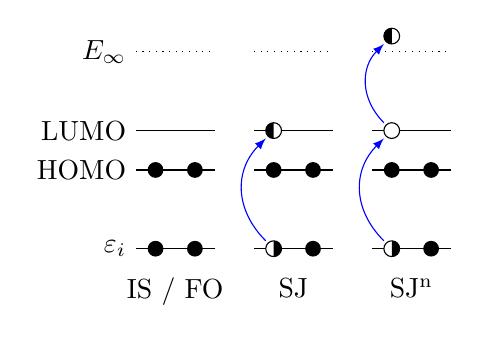
\begin{tikzpicture}
			\draw (0,0) node[left]{$\varepsilon_i$}-- node[midway,below=.25cm]{IS / FO} +(1,0);
			\draw (0,1) node[left]{HOMO}-- +(1,0);
			\draw (0,1.5) node[left]{LUMO}-- +(1,0);
			\draw[dotted] (0,2.5) node[left]{$E_\infty$}-- +(1,0);
			\fill (.25,0) circle (.1cm);
			\fill (.75,0) circle (.1cm);
			\fill (.25,1) circle (.1cm);
			\fill (.75,1) circle (.1cm);
			
			\begin{scope}[xshift=1.5cm]
				\draw (0,0) -- node[midway,below=.25cm]{SJ} +(1,0);
				\draw (0,1) -- +(1,0);
				\draw (0,1.5) -- +(1,0);
				\draw[dotted] (0,2.5) -- +(1,0);
				\draw[fill=white] (.25,0) circle (.1cm);
				\fill (.25,-.1) arc (-90:90:.1);
				\fill (.75,0) circle (.1cm);
				\fill (.25,1) circle (.1cm);
				\fill (.75,1) circle (.1cm);
				\draw[fill=white] (.25,1.5) circle (.1cm);
				\fill (.25,1.4) arc (-90:-270:.1);
				\draw[-latex,blue] (.15,.1) .. controls +(-.4,.4) and +(-.4,-.4) .. (.15,1.4);
			\end{scope}
			
			\begin{scope}[xshift=3cm]
				\draw (0,0) -- node[midway,below=.25cm]{SJ\textsuperscript{n}} +(1,0);
				\draw (0,1) -- +(1,0);
				\draw (0,1.5) -- +(1,0);
				\draw[dotted] (0,2.5) -- +(1,0);
				\draw[fill=white] (.25,0) circle (.1cm);
				\fill (.25,-.1) arc (-90:90:.1);
				\fill (.75,0) circle (.1cm);
				\fill (.25,1) circle (.1cm);
				\fill (.75,1) circle (.1cm);
				\draw[fill=white] (.25,1.5) circle (.1cm);
				\draw[-latex,blue] (.15,.1) .. controls +(-.4,.4) and +(-.4,-.4) .. (.15,1.4);
				\draw[-latex,blue] (.15,1.6) .. controls +(-.3,.3) and +(-.3,-.3) .. (.15,2.6);
				\draw[fill=white] (.25,2.7) circle (.1cm);
				\fill (.25,2.6) arc (-90:-270:.1);
			\end{scope}
		\end{tikzpicture}
		\caption{Approaches to compute BE as the energy of the molecular orbital where the core hole is located: initial state (IS, also referred to as frozen orbitals, FO) and Slater-Janak (SJ). When the electron is further removed from the system (and conceptually pushed to the vacuum, $E_\infty$), JS\textsuperscript{n} is noted. Adapted from Ref.~\citenum{pueyobellafontPredictingCoreLevel2017}.}
		\label{fig:method}
	\end{figure}
	
After the calculation, the corresponding eigenvalue, $\varepsilon_i\left(\frac{1}{2}\right)$, is extracted. The binding energy is then calculated as:
\begin{equation}
	\text{BE}_i = 
	E_{ref}- \varepsilon_i\left(\tfrac{1}{2}\right), \label{eq:xpsbe}
\end{equation}
where $E_{ref}$ is a reference energy, chosen to ensure consistency across systems. Different choices exists in the literature, and thus this study considers several choices for $E_{ref}$:
\begin{enumerate}
	\item $E_{ref}=0$, thus using only the orbital energy,
	\item $E_{ref}=E_F$, where the Fermi energy $E_F$ is used, computed with \texttt{EFERMI = MIDGAP} in the VASP input to account for Gaussian smearing,
	\item $E_{ref}=E_\infty$, the vacuum energy, calculated by taking the electrostatic potential in the vacuum region of the cell (when dipole correction are included, the vacuum potential is not equal in both side of the slab, the average value is considered),
	\item $E_{ref}=\phi$, where the work function of the system $\phi = E_\infty - E_F$ is considered\cite{kahnFermiLevelWork2015}, and
	\item $E_{ref}= \varepsilon_{ref}$, where $\varepsilon_{ref}$ is the orbital energy of another atom in the cell. Although it might seem reasonable to use calcium, which is present in all slabs, this approach would depend on the slab's nature and would be not possible for gas-phase molecules. To overcome this, an Argon atom (to mimic calcium) is placed in the vacuum region, and $\varepsilon_{ref}=\varepsilon_{Ar,2s}$.
\end{enumerate}
Thus, computing a binding energy for a given atom requires to select a computational protocol, which includes the choice of a  way to deal with the electron reorganization  (in this work, SJ or SJ\textsuperscript{n}), and a $E_{ref}$.
It should be noted, however, that extracting $E_\infty$ is not feasible for bulk systems, where no vacuum region exists, or for charged systems, where the electrostatic potential is not constant in the vacuum region. This latter condition occurs when employing the SJ\textsuperscript{n} method. It is however possible to correct the Fermi level energy to remove the impact of the background of charge, as discussed in Ref.~\citenum{lozovoiInitioSimulationCharged2001}. This possibility is referred to as $E_{ref}=E_F'$, where $E_F' = E_F - \max\{E_{elst}(z)\}$, with $E_{elst}(z)$ being the planar average of the electrostatic potential along the $z$ axis.

Finally, while the determination of absolute binding energies (BE) is challenging from a theoretical perspective, the measurement or calculation of the work function, $\phi$ in Eq.~\eqref{eq:xps}, is also complex. As a result, both experimentalists and quantum chemists often focus on the relative binding energy, $\Delta\text{BE}$, which is the difference in binding energy for a given atom with respect to a reference compound \cite{vinesPredictionCoreLevel2018}. In this contribution, relative BE values are computed as:\begin{equation}
	\Delta\text{BE}_i = \text{BE}_i - \text{BE}(\text{ref}), \label{eq:dbe}
\end{equation} 
using the calculated or experimental BE values for \ce{CH4}, \ce{NH3}, \ce{H2O}, \ce{B2H6}, and \ce{HF} as references for carbon, nitrogen, oxygen, boron, and fluorine, respectively. The experimental values are taken from Ref.~\citenum{pueyobellafontPredictingCoreLevel2017}. For calcium, the value for bulk Ca in CaO is used, taken from the XPS library \cite{cristXPSLibraryWebsite2021a} (computationally, a  2x2 slab containing 16 layers is used).

	
\section{Computational details}

All calculations (optimization and binding energies) were performed using the PBE-D3 level of theory with VASP (version 6.4.1) and the projector-augmented wave (PAW) method \cite{blochlProjectorAugmentedwaveMethod1994}. The energy convergence criterion was set to \SI{e-4}{\electronvolt}, with a cutoff of \SI{550}{\electronvolt} for the kinetic energy of the plane waves. Gaussian smearing of the energy of valence electrons, with a width of \SI{0.2}{\electronvolt}, was applied. Brillouin zone integration was performed at the $\Gamma$-point for molecules in the gas phase, using a 4x4x4 Monkhorst-Pack k-point mesh\cite{monkhorstSpecialPointsBrillouinzone1976} for bulk calculations, and a 4x4x1 mesh for slab calculations. The \texttt{Ca\_sv} pseudopotential\cite{blochlProjectorAugmentedwaveMethod1994,kresseUltrasoftPseudopotentialsProjector1999} was employed to model calcium.

\paragraph{Geometry optimization.} All optimizations were carried out using the Limited-memory Broyden-Fletcher-Goldfarb-Shanno  (L-BFGS) algorithm, driven by the Atomic Simulation Environment (ASE) package \cite{larsenAtomicSimulationEnvironment2017}, using VASP energies and forces as inputs, until the force on all atoms was below \SI{e-2}{\electronvolt\per\angstrom}.

In gas phase, each molecule was placed in a cubic box with a side length of \SI{20}{\angstrom} (with the molecule center of mass placed at the origin) and optumized (with frozen cell parameters).

In order to build slabs, bulk \ce{Ca^0} (from the Material Project, \texttt{MP-45}), CaO (\texttt{MP-2605}), and \ce{CaH2} (\texttt{MP-23713}) were selected, and their atomic positions and cell parameters were optimized. Subsequently, to determine the optimal surface orientation, 1x1 slabs with increasing thickness along different low-index orientations [(100), (110), and (111)] were constructed using ASE \cite{larsenAtomicSimulationEnvironment2017}. The slabs were relaxed with the central two layers frozen to mimic bulk conditions, with the distance between slab repetitions set to 10 times the $c$ cell parameter of the bulk. For each orientation, the surface energy $\gamma^{hkl}$ was calculated by least-squares fitting of the following expression \cite{sunEfficientCreationConvergence2013,tranSurfaceEnergiesElemental2016}:
\begin{equation}
	E^{hkl}(N) = E_0\,N + 2A\,\gamma^{hkl} \label{eq:surf}
\end{equation}
where $N$ is the number of layers in the slab, $A$ is the slab surface area, $E^{hkl}(N)$ is the energy of the relaxed slab cut along $(hkl)$, and $E_0$ approximates the energy of one layer. The results (Table \ref{tab:surf}, Fig.~S2) indicate that (100) surfaces are the most energetically favorable, consistent with the literature \cite{deleeuwDensityFunctionalTheory2000,ebadiInsightsLiMetalOrganic2019}. 
Thus, using these (100) orientation, 3x3 (\ce{Ca^0} and CaO) and 2x2 (\ce{CaH2}) slabs (ensuring a slab surface of $\sim 10\times \SI{10}{\angstrom}$) consisting of 6 layers, with a vacuum of \SI{20}{\angstrom} between two slab repetitions were created and relaxed (with frozen cell parameters). 

Additionally, given that it reported to be favorable\cite{deleeuwDensityFunctionalTheory2000,fujimoriInteractionWaterCaO2016a}, the adsorption of water on the CaO surface was investigated. In fact, the contamination of CaO by surface hydroxyls was reported in many experiments\cite{dupinSystematicXPSStudies2000,bebenseeAdsorptionOxygenWater2008,fujimoriInteractionWaterCaO2016a,cristXPSLibraryWebsite2021a}. Thus, an additional slab with full coverage (1 water molecule per surface Ca), denoted as \ce{CaO.H_2O}, was built and its geometry was also optimized. 

\begin{table}[!h]
	\centering
	\begin{tabular}{lccc}
		\toprule
		&	\ce{Ca^0} & \ce{CaO} &	\ce{CaH2} \\
		\midrule
		(100) & 0.555 ($N\in[6,16]$) & 0.470 ($N\in[6,16]$) & 0.871  ($N\in[12,32]$)\\
		(110) & 0.630  ($N\in[6,16]$)& 1.777  ($N\in[6,16]$)& 1.109 ($N\in[12,32]$)\\
		(111) & 0.563  ($N\in[6,16]$) & 4.080  ($N\in[5,15]$)  & 1.117   ($N\in[12,32]$) \\ 
		\bottomrule
	\end{tabular}
	\caption{Surface energies ($\gamma^{hkl}$, in \si{\joule\per\meter\squared}) of Ca, CaO, and \ce{CaH2} slabs along different orientations, as determined through Eq.~\eqref{eq:surf} using the $N$ values given in parentheses.}
	\label{tab:surf}
\end{table}

Finally, compounds \textbf{a}--\textbf{j} (Fig.~\ref{fig:THFdegradation}) were positioned on both sides of the slabs, initially placed approximately \SI{6}{\angstrom} from the surface. A final optimization was then performed, keeping the cell parameters and the two central layers fixed.

\paragraph{Binding energies.}  VASP allows targeting a specific orbital, $i$, by removing half an electron from it. For SJ calculation, dipole corrections (using the \texttt{IDIPOL} keyword) are included. For SJ\textsuperscript{n} calculations, it is necessary to adjust the total number of valence electrons (by default, half an electron is added; see Fig.~\ref{fig:method}) using the \texttt{NELECT} keyword. However, it is not possible to account for spin-orbit coupling in such calculations, and therefore we limit ourselves to the study of 1s and 2s binding energies. To simulate a spectrum, a Gaussian function centered at each computed \dbe{} is used. Unless otherwise specified, a full width at half maximum (FWHM) of \SI{0.5}{\electronvolt} is employed.

To evaluate the accuracy of the different computational protocols (SJ and SJ\textsuperscript{n} methods, as well as the choice of $E_{ref}$), two sets of calculations were conducted. First, the results from Belafont \textit{et al.} \cite{pueyobellafontPredictingCoreLevel2017}, which compare experimental and theoretical gas-phase \dbe{} values (computed at the same level of approximation as this study), were replicated. Their dataset includes 184 experimental absolute binding energies (BEs) from 68 molecules, covering carbon ($N=107$), nitrogen ($N=20$), oxygen ($N=22$), boron ($N=20$), and fluorine ($N=15$) atoms (Fig.~S1). Each molecule was placed in a cubic box with a side length of \SI{20}{\angstrom}, centered at the molecule's center of mass. The \dbe{} values were then computed for each atom of interest. Other parameters, such as vacuum energy, were extracted from the density (\texttt{CHGCAR}) and potential (\texttt{LOCPOT}) files. For calculations involving an additional argon atom, it was positioned at the center of the box.

In parallel, the effect of slab thickness was examined using the bare slabs of increasing thickness described above. Binding energies were calculated on 2x2 slabs with a (100) orientation, separated by an interslab distance of \SI{20}{\angstrom}. The geometries were based on the optimized 1x1 slabs from the surface energy study, with a supercell created and then adjusting the interslab spacing. The \dbe{} values were computed for each atom of interest, and the relevant parameters were extracted accordingly. For calculations involving an additional argon atom, placed in a cell where the slab is positioned at the center, the argon atom was located at the origin.

Finally, the \dbe{} values were calculated for each atom of interest in the molecules grafted onto the various surfaces, using the selected reference energy. It is important to note that, in these calculations with the SJ protocol, the relatively small surface area of the slabs may introduce artifacts due to the periodic repetition of core holes in close proximity, especially for adsorbates that are far from the surface\cite{taucherFinalStateSimulationsCoreLevel2020}. Although larger supercells could be employed to mitigate this issue, doing so would significantly increase computational time.



\section{Results}

\NewDocumentCommand{\cp}{O{}m}{SJ\IfNoValueTF{#1}{}{\textsuperscript{#1}}+$E_{ref} = #2$}

\subsection{Selection of a computational protocol for binding energies}

A comparison between experimental and computed \dbe{} values for carbon is shown in Fig.~\ref{fig:xps_C185_C}. Consistent with previous studies \cite{pueyobellafontPredictingCoreLevel2017,golzeAccurateAbsoluteRelative2020}, the \cp[n]{0} protocol provides reliable results for all atoms, exhibiting a very small mean error and an acceptable standard deviation. However, achieving this level of agreement requires using a reference per atom (Table S1), as the discrepancy between experimental and computed absolute BEs tends to increase with the atomic number. Similarly, using \cp[n]{\varepsilon_{Ar,2s}} results in small errors. Across the entire set of 184 \dbe{} values, the combination of each reference energy with the SJ\textsuperscript{n} approach yields comparable results (Fig.~\ref{fig:xps_C185}). 

In contrast, other reference energies significantly degrade the accuracy of the predicted gas-phase \dbe{}. The largest errors are observed when using the Fermi energy, \cp{E_F}, \cp[n]{E_F}, or \cp [n]{E_F'}. In combination with the SJ\textsuperscript{n} protocol it leads to underestimated \dbe{} values. Then, \cp{0}, \cp{\varepsilon_{Ar,2s}}, and \cp{E_\infty} perform similarly, and finally, the lowest error found when using \cp{\phi}, although it remains substantial. Moreover, all reference energies combined with the SJ protocol tend to overestimate the \dbe{} values.

\textbf{but why?}


\begin{figure}[!h]
	\centering
	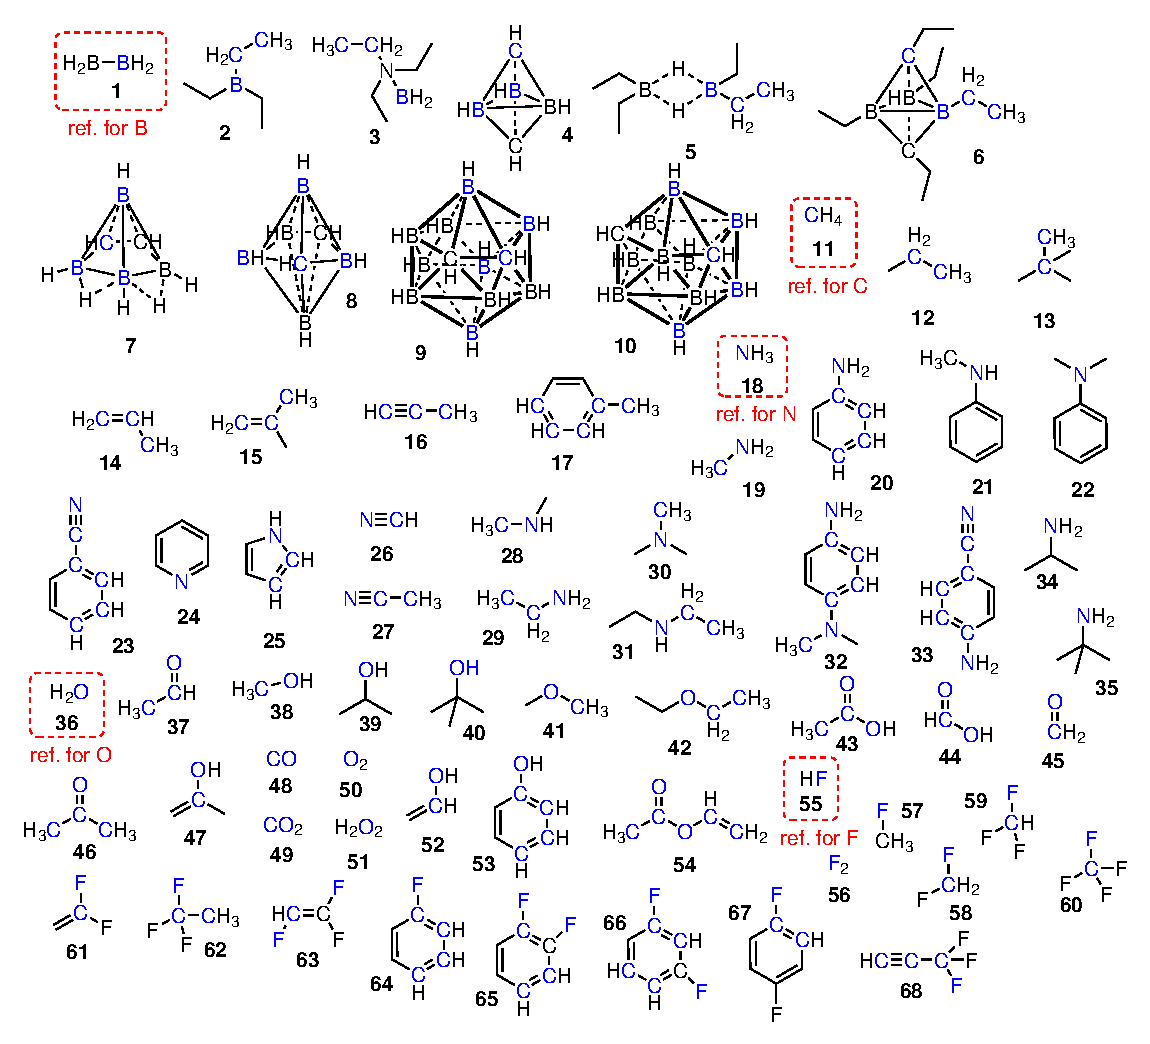
\includegraphics[width=\linewidth]{Figure3}
	\caption{Error in the calculated gas-phase \dbe{}  (in \si{\electronvolt}) with respect to experiment, computed using the SJ (left) and SJ\textsuperscript{n} (right) method and different reference energies, for the carbon atom ($N=107$). For each reference, the violin plot illustrates the error distribution (horizontal lines represent, from bottom to top, the minimum, 1\textsuperscript{st} quartile, median, 3\textsuperscript{rd} quartile, and maximum). Additionally, the mean $\pm$ standard deviation is displayed}
	\label{fig:xps_C185_C}
\end{figure}


\begin{figure}[!h]
	\centering
	\includegraphics[width=.85\linewidth]{Figure4}
	\caption{Comparison between experimental and calculated gas phase \dbe{} (in \si{\electronvolt}), as computed with thetwo best-performing protocols, on the different atoms. For each of them, the error (as mean $\pm$ standard deviation) is given.}
	\label{fig:xps_C185}
\end{figure}


\clearpage

The situation differs for slabs. The impact of slab thickness ($N$) on the Ca 2s binding energy, evaluated using both protocols, is shown in Figs.~\ref{fig:slabsthicknessSJ}--\ref{fig:slabsthicknessSJn}. The results reveal a substantial difference (exceeding \SI{0.5}{\electronvolt} for certain reference energies) between the surface layers (defined as the first and last layers of the slab) and the bulk \dbe{}, with relatively small standard deviation (values are provided in Tables S3-S4). With all protocols, BE(surface Ca 2s) $>$ BE(bulk Ca 2s). Due to the different environments, this was expected \textbf{Y'a probablement des papiers discutant du lien entre morphologie de la surface et XPS}. 

Another key observation is that slab thickness influences some results more than others. For calculations with \cp{E_F}, \cp{\varepsilon_{Ar,2s}}, and \cp{E_\infty}, the predicted values remain nearly constant as $N$ increases. Conversely, the SJ\textsuperscript{n} method appears very sensitive to the system size. It should however be noted that with $E_{ref}=\varepsilon_{Ar,2s}$, calculation fails to converge or provide slightly different values, resulting in large standard deviations, notably for CaO with $N=16$ layers. 

For O 1s, as illustrated in Fig.~\ref{fig:slabOH2}, where simulated XPS spectra for CaO and \ce{CaO.H2O} (both with 6 layers) are shown, the distinction between bulk and surface contributions is notable. In the case of CaO, BE(bulk O 1s in CaO) $>$ BE(surface O 1s in CaO), whereas in \ce{CaO.H2O}, the reverse trend is observed, consistent across all protocols. Furthermore, BE(bulk O 1s in CaO) $\approx$ BE(bulk O 1s in \ce{CaO.H2O}) when using \cp{E_F}, \cp{E_\infty}, or \cp{\varepsilon_{Ar,2s}}. However, the latter yields unreliable results, as evidenced by the spurious peak at \dbe{} = \SI{0}{\electronvolt} in the O 1s spectra, suggesting an artificial differentiation between hydroxyl environments that is not reflected when using other reference energies. Finally, for the hydroxylated slabs, BE(surface O 1s) $\approx$ BE(hydroxyl O 1s) with most protocols.



\begin{figure}[!h]
	\centering
	\includegraphics[width=.85\linewidth]{Figure5}
	\caption{Effect of slab thickness (expressed as the number of layers, $N/N_0$, where $N_0 = 2$ for \ce{Ca^0} and CaO and 4 for \ce{CaH2} represents the number of layers in the unit cell) on the mean bulk (filled markers) and surface (empty markers) \dbe{} for Ca 2s (in \si{\electronvolt}), calculated using the SJ method and various reference energies. The vertical lines indicate standard deviation.}
	\label{fig:slabsthicknessSJ}
\end{figure}

\begin{figure}[!h]
	\centering
	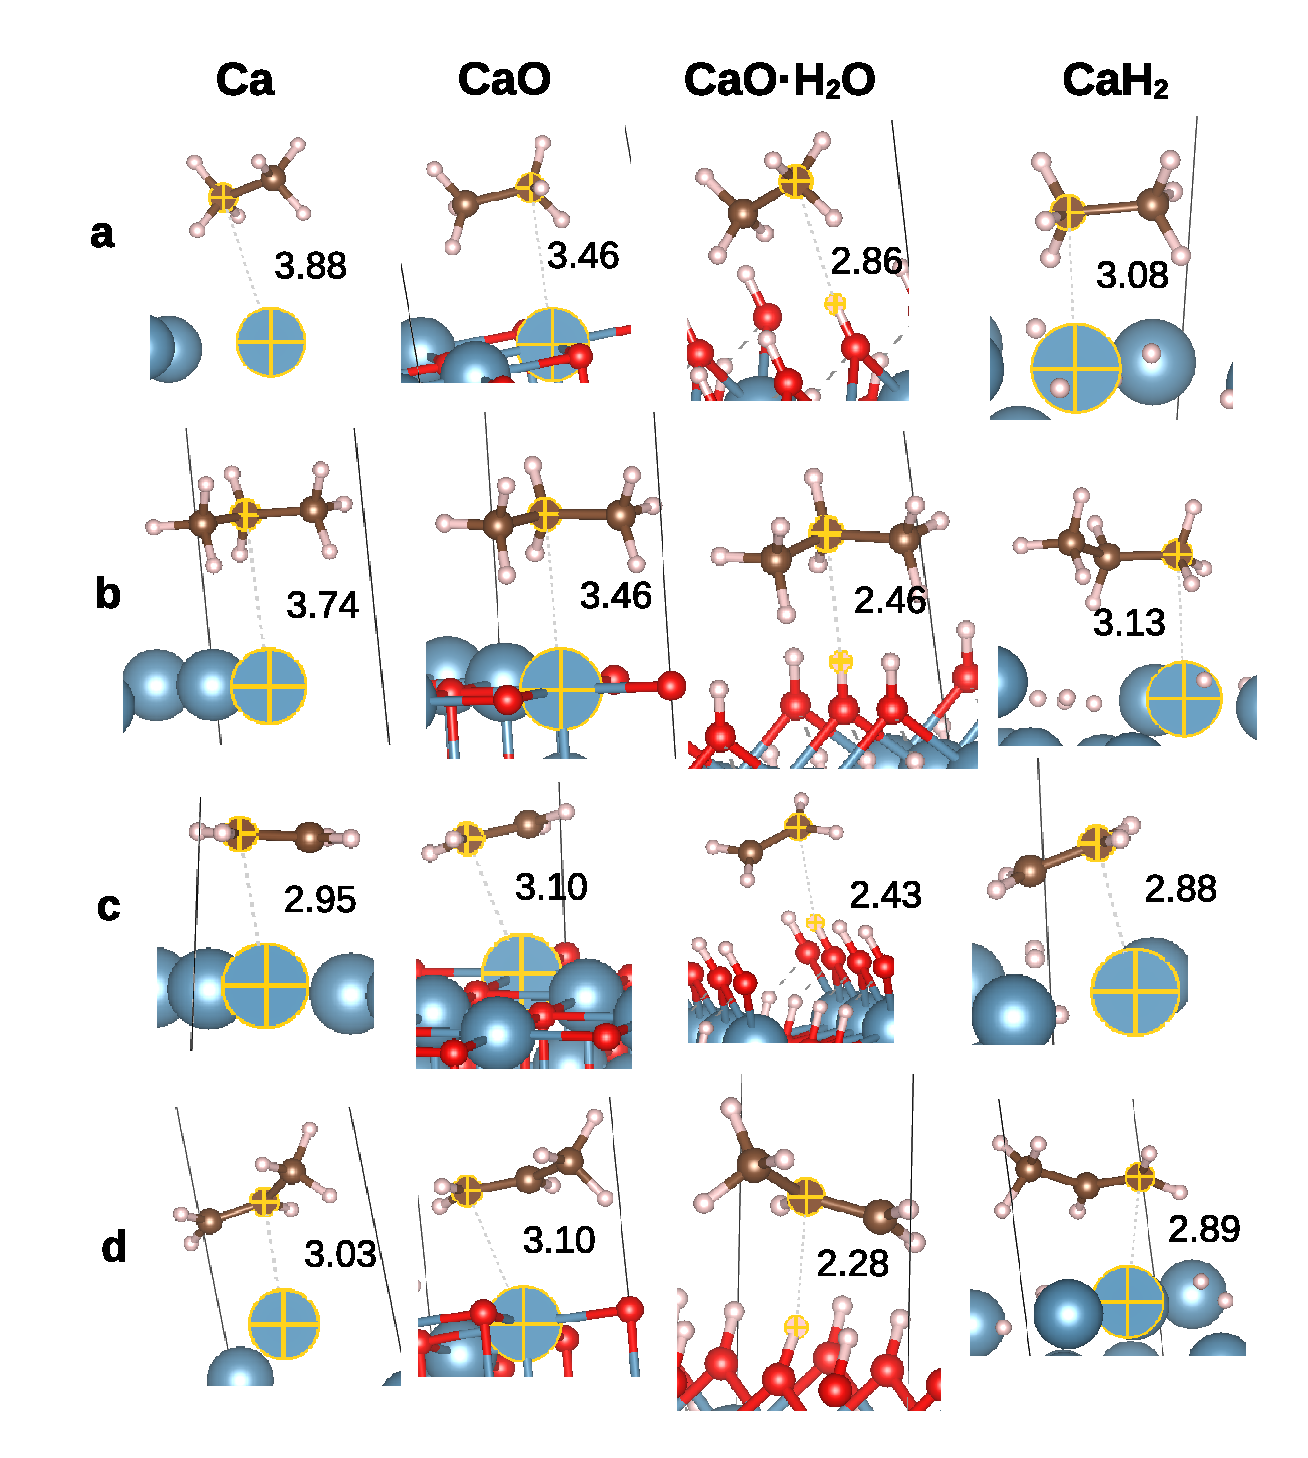
\includegraphics[width=.85\linewidth]{Figure6}
	\caption{Effect of slab thickness (expressed as the number of layers, $N/N_0$, where $N_0 = 2$ for \ce{Ca^0} and CaO and 4 for \ce{CaH2} represents the number of layers in the unit cell)  on the mean bulk (filled markers) and surface (empty markers) \dbe{} for Ca 2s (in \si{\electronvolt}), calculated using the SJ\textsuperscript{n} method and various reference energies. The vertical lines indicate standard deviation.}
	\label{fig:slabsthicknessSJn}
\end{figure}


\begin{figure}[!h]
	\centering
	\includegraphics[width=\linewidth]{Figure7a}
	\includegraphics[width=\linewidth]{Figure7b}
	\caption{Effect of the reference energy on the simulated XPS spectra of CaO (dashed line)  and \ce{CaO.H2O} (plain line), calculated using the different protocols. Letters indicate mean values for bulk (``b"), surface (``s"), and surface hydroxides (``h", only for \ce{CaO.H2O}  O 1s).}
	\label{fig:slabOH2}
\end{figure}

Experimentally, XPS spectra for calcium metal slabs and their oxides, including Ca 2s binding energies, are scarce. Some values from various sources are summarized in Table S2. To the best of our knowledge, no reported measurements exist for \ce{CaH2}, and data for other peaks are limited \cite{franzenXPSSpectraCrystalline1977,sveinbjornssonIonicConductivityFormation2014}. Moreover, due to calcium's high reactivity, contamination by oxides, hydroxyls, and hydrocarbons complicates the analysis \cite{dupinSystematicXPSStudies2000,bebenseeAdsorptionOxygenWater2008,fujimoriInteractionWaterCaO2016a,cristXPSLibraryWebsite2021a}. Nonetheless, two trends can be discerned: \begin{inparaenum}[(i)]
	\item unlike the preceding alkaline earth metal, magnesium \cite{dobrovolskyXPSStudyInfluence2017}, recent data suggest that BE(Ca 2s in \ce{Ca^0}) $>$ BE(Ca 2s in CaO) $\approx$ BE(Ca 2s in \ce{CaO.H2O}) \cite{ochsCO2ChemisorptionCa1998,cristHandbookMonochromaticXPS2000a,cristXPSLibraryWebsite2021a}, and 
	\item BE(Bulk O 1s in CaO) $\approx$ BE(bulk O 1s in \ce{CaO.H2O}) $<$ BE(hydroxyls O 1s in \ce{CaO.H2O}) \cite{dupinSystematicXPSStudies2000,bebenseeAdsorptionOxygenWater2008,fujimoriInteractionWaterCaO2016a,cristXPSLibraryWebsite2021a}.
\end{inparaenum}
Only the \cp{E_\infty} protocol satisfies these two criteria, although it globally underestimate the \dbe{} for O 1s (which is, \textit{e.g.}, smaller than \SI{-7}{\electronvolt} for bulk CaO\cite{cristXPSLibraryWebsite2021a}).

Consequently, a consistent treatment of both gas-phase systems and slabs using the same method is not feasible in this work.


\clearpage

\subsection{Adsorption on slab: geometrical and energetic aspects}

The optimized geometries of compounds \textbf{a}–\textbf{j}, following their adsorption on the slabs, are depicted in Figs.~\ref{fig:distsad}–\ref{fig:distsj}. The interaction energy, calculated as $\Delta E_{int} = E_{2X@Y} - E_Y - 2E_X$ (where $E_X$ represents the energy of a single adsorbate, placed on each side of the slab, and $E_Y$ is the energy of the substrate), is presented in Table~\ref{tab:int}. Note that no thermochemical corrections (e.g., zero-point vibrational energy) have been applied in these calculations.




\begin{figure}[!b]
	\centering
	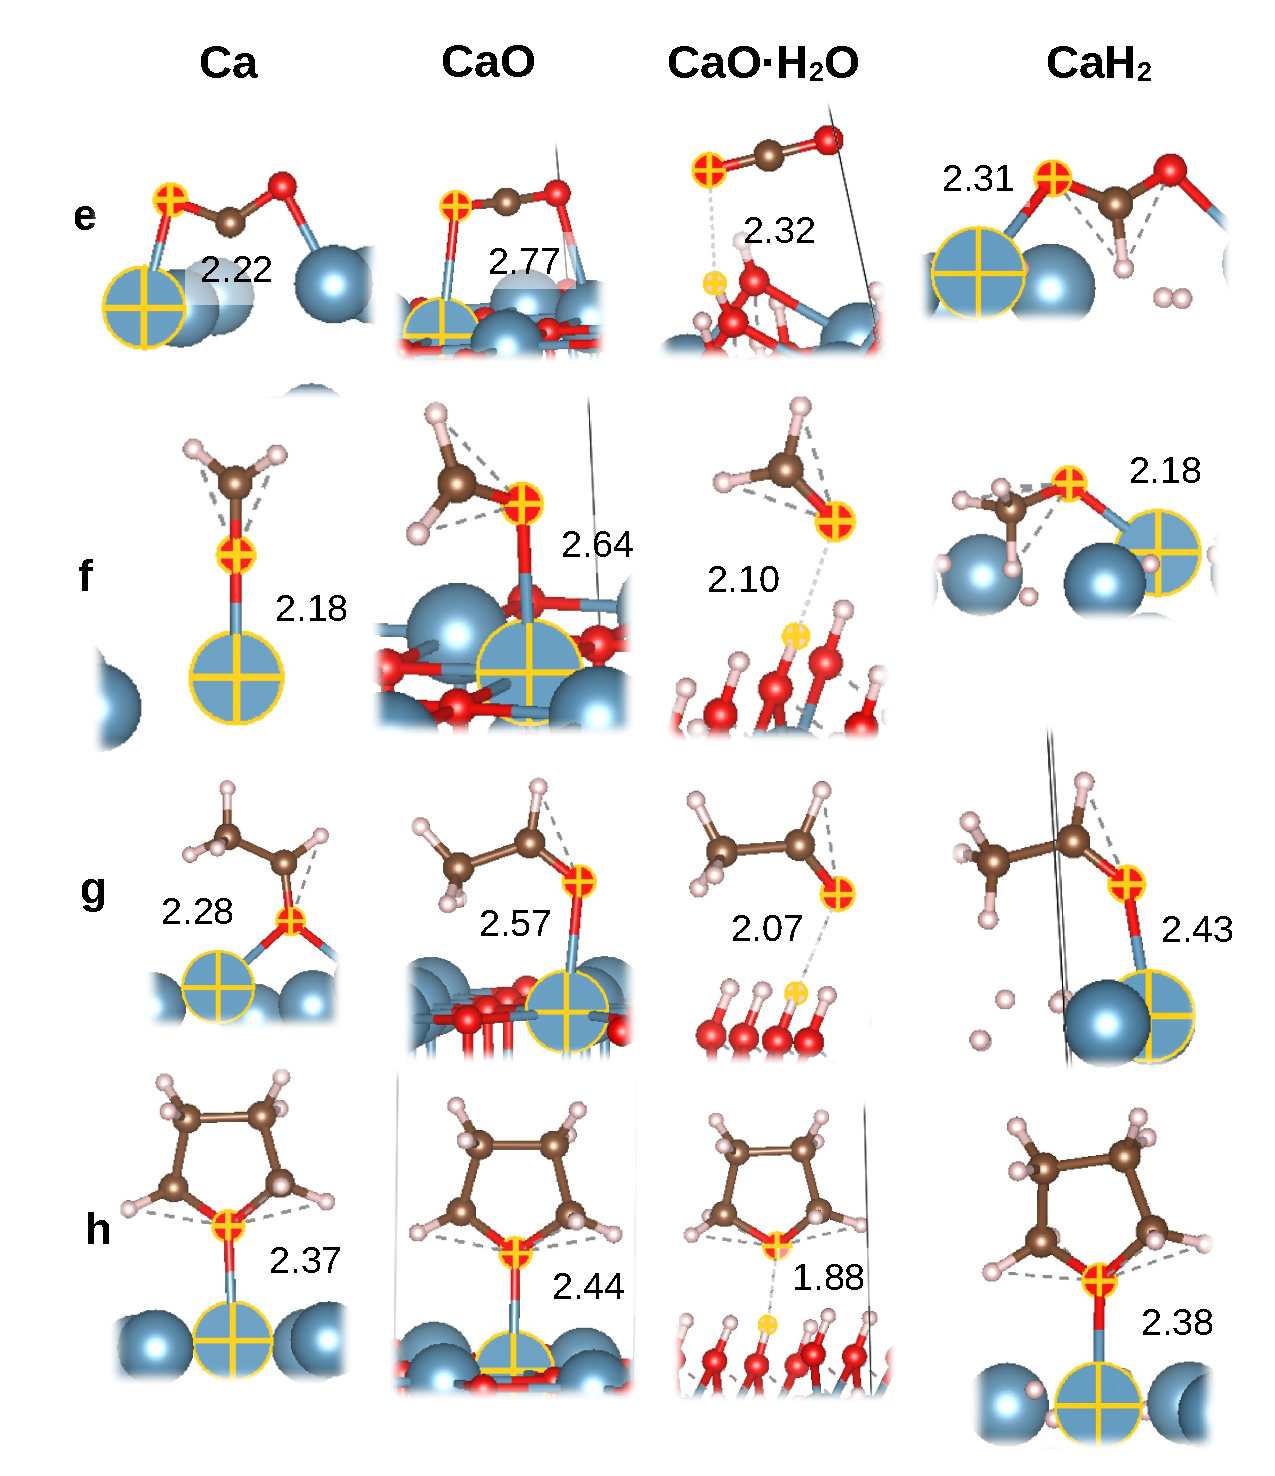
\includegraphics[width=\linewidth]{Figure8}
	\caption{Geometrical structures of the adsorbate (hydrocabrons, \textbf{a}-\textbf{d}) + substrates systems, after geometry optimization, described by representative intermolecular distances (in \si{\angstrom}).}
	\label{fig:distsad}
\end{figure}

\begin{figure}[!h]
	\centering
	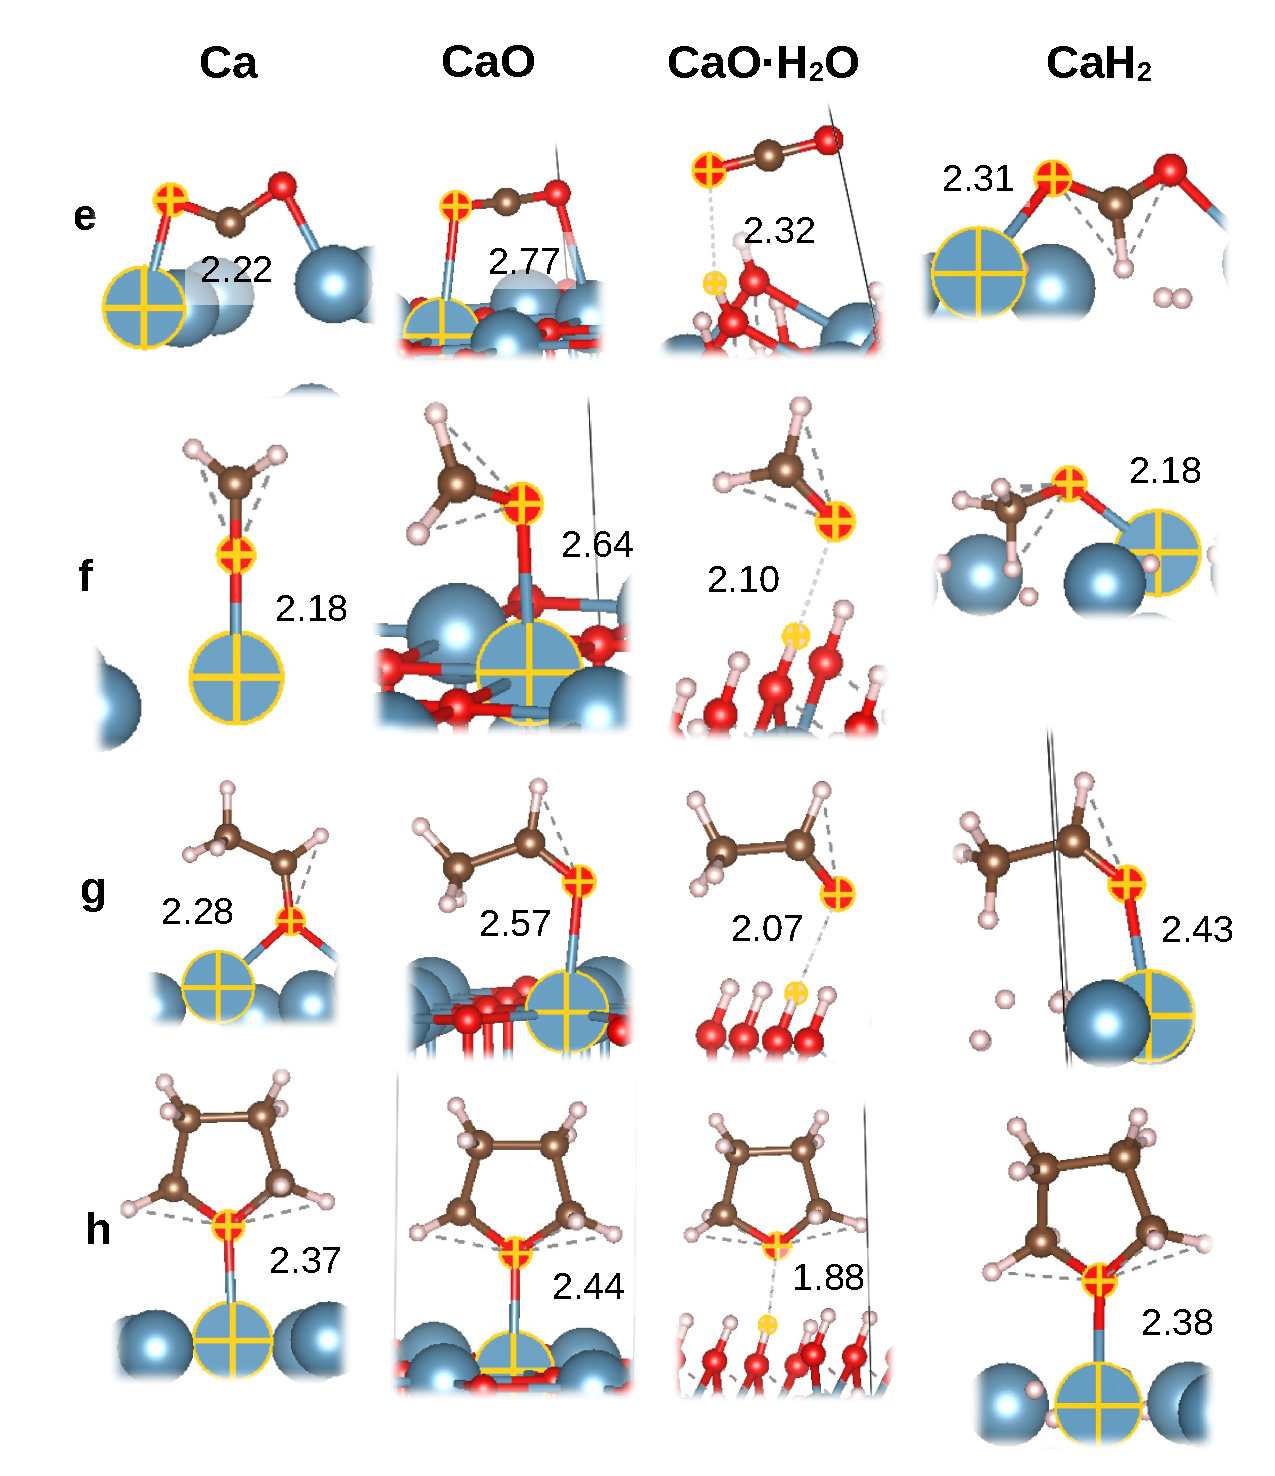
\includegraphics[width=\linewidth]{Figure9}
	\caption{Geometrical structures of the adsorbate (carbohydrates, \textbf{e}-\textbf{i}) + substrates systems, after geometry optimization, described by representative intermolecular distances (in \si{\angstrom}).}
	\label{fig:distsei}
\end{figure}

\begin{figure}[!h]
	\centering
	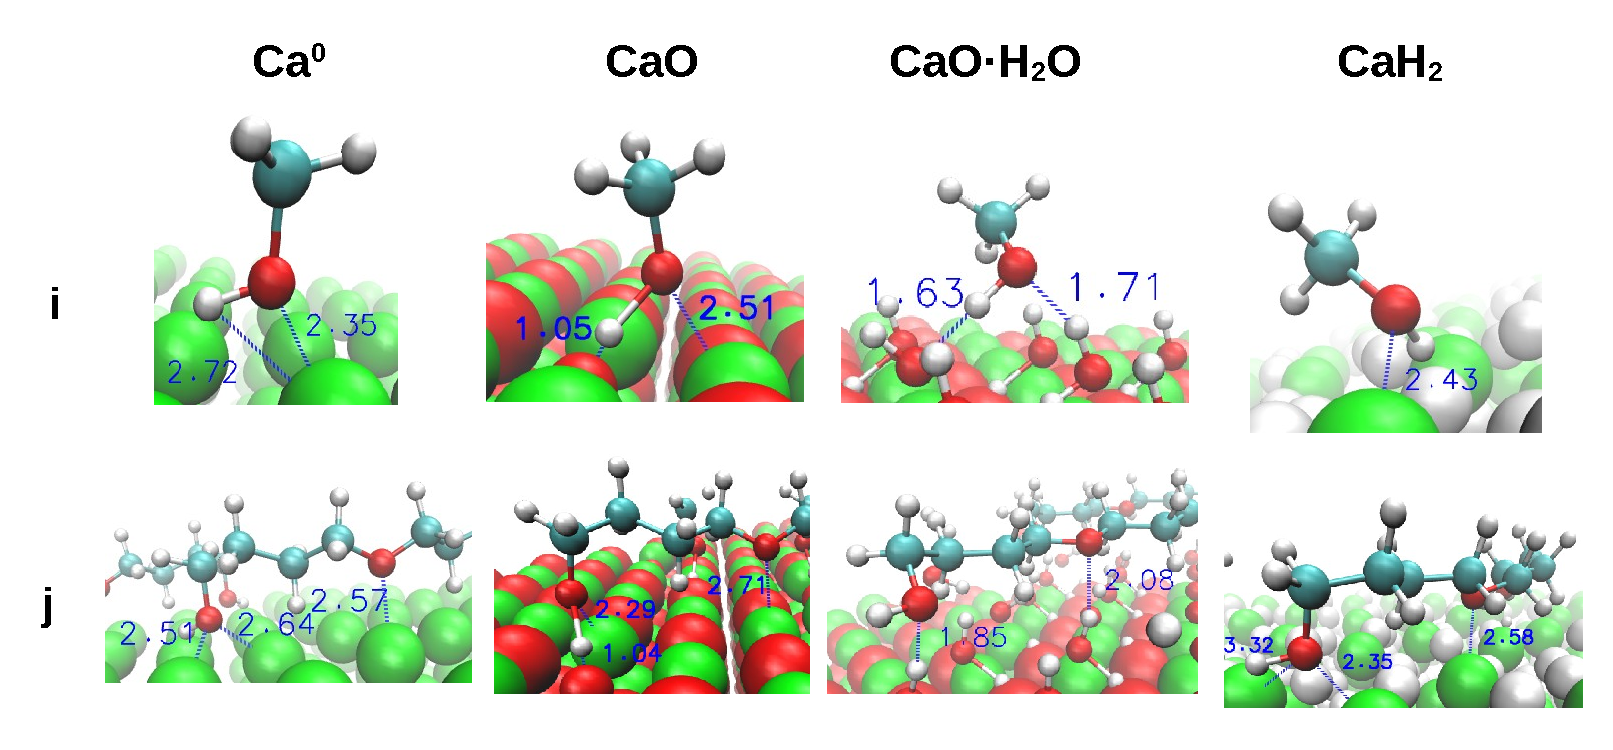
\includegraphics[width=.7\linewidth]{Figure10}
	\caption{Geometrical structures of the adsorbate (\textbf{j}) + substrates systems, after geometry optimization, described by representative intermolecular distances (in \si{\angstrom}).}
	\label{fig:distsj}
\end{figure}

\begin{table}[!h]
	\centering
	\begin{tabular}{>{\bfseries}lcccc}
		\toprule
		& Ca & \ce{CaO} & \ce{CaO.H2O} & \ce{CaH2} \\
		\midrule
		& \multicolumn{4}{c}{Hydrocarbons} \\
		a & -0.67 & -0.44 & -0.65 & -0.41 \\
		b & -0.42 & -0.63 & -0.87 & -0.52 \\
		c & -0.95 & -0.34 & -0.78 & -0.80 \\
		d & -1.04 & -0.53 & -0.98 & -0.84 \\
		\midrule
		& \multicolumn{4}{c}{Polar carbohydrates} \\
		e & -2.03 & -0.37 & -0.67 & -6.42 \\
		f & -3.21 & -0.41 & -0.97 & -1.99 \\
		g & -1.52 & -0.70 & -1.18 & -2.72 \\
		h & -1.62 & 2.08 & -1.31 & -1.61 \\
		\midrule
		& \multicolumn{4}{c}{Protic carbohydrates} \\
		i & -1.81 & -1.60 & -2.19 & -1.64 \\
		j & -4.53 & -2.54 & -5.60 & -4.31 \\
		\bottomrule
	\end{tabular}
	\caption{Interaction energy ($\Delta E_{int}$, in \si{\electronvolt}) between the adsorbate and the substrate.}
	\label{tab:int}
\end{table}

There are three primary modes of interaction between the substrate and the adsorbate: \begin{inparaenum}[i)] \item van der Waals (vdW) forces, 
\item hydrogen bonding (HB), and 
\item chemisorption. 
\end{inparaenum}
First, hydrocarbons (\textbf{a}–\textbf{d}) mainly interact through vdW forces, as indicated by the relatively large distances between the adsorbate and substrate (Fig.~\ref{fig:distsad}) and the low interaction energies ($E_{int} < \SI{1}{\electronvolt}$). However, for unsaturated hydrocarbons (\textbf{c}-\textbf{d}), the distances are shorter ($\sim\SI{3}{\angstrom}$) compared to saturated ones (\textbf{a}-\textbf{b}) on the \ce{Ca^0}, \ce{CaO.H2O}, and \ce{CaH2} slabs, leading to slightly higher interaction energies.

Second, HB interactions are prevalent between \ce{CaO.H2O} and carbohydrates (\textbf{e}-\textbf{j}). From \textbf{e} to \textbf{j}, interaction energies increase, which correlates with a decrease in the oxygen(substrate)--hydrogen(slab) distance. In protic hydrocarbons (\textbf{i}-\textbf{j}), HB formation occurs between the hydrogen of the substrate and the oxygen of the slab.

Lastly, carbohydrates can exhibit significant interaction energies ($> \SI{1}{\electronvolt}$) with the \ce{Ca^0} and \ce{CaH2} slabs, particularly due to oxygen--calcium interactions, accompanied by small interatomic distances, suggesting chemisorption. This is especially pronounced for \ce{CO2} (\textbf{e}) and \ce{CH2=O} (\textbf{f}) on the \ce{CaH2} slab, where both compounds undergo an increase in hybridization (\textit{e.g.}, from \ce{sp^2} to \ce{sp^3} for \textbf{f}), facilitated by interaction with a slab's hydrogen.
Interestingly, the CaO slab follows a different trend. While interactions with polar carbohydrates (\textbf{e}–\textbf{h}) result in low or even slightly positive (\textbf{h}) interaction energies (similar to vdW), protic carbohydrates (\textbf{i}-\textbf{j}) show small hydrogen(substrate)--oxygen(slab) distances, suggesting proton transfer between the substrate and slab.

These observations provide insights into potential degradation mechanisms. The proton transfers on the CaO surface support the hypothesis of hydroxyl formation on the slab. Moreover, reactions involving hydrogen from the \ce{CaH2} slab indicate possible surface instability under certain conditions.

\clearpage
\subsection{Binding energies of adsorbate on slabs}

Since directly comparing molecules in the gas phase with those adsorbed on a slab is methodologically questionable (\textit{vide infra}), the binding energies before and after adsorption will be discussed. For the former, the geometries where the molecules are \SI{6}{\angstrom} from the slab surface are used. The XPS spectra of the adsorbates (computed using the results where these molecules are on top of bare Ca) are analyzed in Fig.~\ref{fig:adsorbare}. The C 1s spectra can be divided into three parts (in agreement with the trends reported in Fig.~\ref{fig:trends}): \begin{inparaenum}[i)]
	\item unsaturated carbons, with the lowest binding energies (\textit{e.g.}, \textbf{c} and \textbf{d}),
	\item aliphatic carbons (\textit{e.g.}, \textbf{a} and \textbf{b}), and
	\item carbons with neighboring oxygen atoms, with the highest binding energies (\textit{e.g.}, \textbf{g}).
\end{inparaenum}
Similarly, the O 1s spectra can be divided into two categories, depending on the hybridization of the oxygen. The lowest binding energies are associated with \ce{C=O} (\textit{e.g.}, \textbf{f} and \textbf{g}).

Two important observations should be noted: first, these binding energies are lower than those predicted in the gas phase.\footnote{Encore une fois, comparaison casse-gueule ;)} It is difficult at this time to determine whether this is due to the methodology (SJ vs. SJ\textsuperscript{n}, $E_F$ or not) or the presence of the Ca slab. One way to address this question would be to study the impact of the distance between the molecule and the slab. Second, the results for \textbf{e} (\ce{CO2}) do not follow the aforementioned trends (its O 1s binding energy is surprisingly large), indicating that further investigation definitely is required (could it be that since it is smaller, it feels less the slab?).

\clearpage

The impact of adsorption on binding energies is detailed in Figs.~\ref{fig:spectraXPSadsab}-\ref{fig:spectraXPSadsij}. For Ca 2s, adsorption-induced changes are minimal, with slightly more noticeable effects on the CaO slab, though not significant enough to be detectable experimentally. However, more substantial changes are observed for the other atoms studied: 
First, interaction with bare Ca results in a shift to lower binding energies in C 1s and a shift to higher binding energies in O 1s (when available), indicating electron transfer between the slab and the adsorbate. This suggests that interactions with hydrocarbons may involve more than just van der Waals forces. Then, hydrogen bond formation at the surface of \ce{CaO.H2O} causes a slight shift to higher O 1s \dbe{}, which increases with the strength of the bond (\textit{e.g.}, \textbf{f}-\textbf{h}).
Furthermore, proton transfers, seen in the interactions between \textbf{e} and \textbf{f} with \ce{CaH2} and between \textbf{i} and \textbf{j} with CaO, lead to significant changes in C 1s and O 1s binding energies, consistent with changes in hybridization. Finally, C 1s binding energies also change when unsaturated hydrocarbons (\textbf{c} and \textbf{d}) interact with \ce{CaH2}, suggesting a modification of the carbon's chemical environment, which may not be immediately apparent when inspecting the geometries.
These findings demonstrate that XPS binding energies are highly sensitive to changes in the chemical environment of the atoms.

\clearpage
\section{Conclusions}
XPS offers valuable insights into the chemical environment of atoms and the changes they undergo during adsorption. However, careful consideration must be given to the methodologies employed, as direct comparisons between results can be challenging due to potential inconsistencies across different systems.

To address these concerns, a thorough assessment of the methodology is necessary. Key considerations include, first, the impact of distance beetween slab and adsorbate The effect of the separation between the slab and the adsorbate on the \dbe{} should be thoroughly investigated. This examination is crucial to establish a clear connection to gas phase results and ensure accurate interpretations.
Then, the application of the SJ\textsuperscript{n} methodology. The SJ\textsuperscript{n} approach should be explored for adsorbates as well. The discussion around Fig.~\ref{fig:slabsthicknessSJn} suggests that SJ\textsuperscript{n} provides a better estimate of \dbe{} for CaO slabs. Confirmation of this finding could improve the reliability of \dbe{} predictions for various systems.

Once the methodology is validated, a deeper analysis of the experimental data provided by Prof. A. Vlad can be undertaken (thought we already have some insights). These data includes spectra for aging over different periods of time, which could provide insights into the kinetics of the degradation process. IR spectroscopy will enhance this analysis, when possible.

Furthermore, another objective is to investigate the behavior of \ce{BH4} and \ce{BF4} ions, aligning with the goals of the ECOBAT project. By integrating these investigations, a comprehensive understanding of the adsorption processes and chemical transformations in these systems can be achieved.


\clearpage
\bibliography{biblio}
	
\end{document}